\chapter{Design}
\label{sec:design}

% Ist das zentrale Kapitel der Arbeit. Hier werden das Ziel sowie die
% eigenen Ideen, Wertungen, Entwurfsentscheidungen vorgebracht. Es kann
% sich lohnen, verschiedene Möglichkeiten durchzuspielen und dann
% explizit zu begründen, warum man sich für eine bestimmte entschieden
% hat. Dieses Kapitel sollte - zumindest in Stichworten - schon bei den
% ersten Festlegungen eines Entwurfs skizziert werden.
% Es wird sich aber in einer normal verlaufenden
% Arbeit dauernd etwas daran ändern. Das Kapitel darf nicht zu
% detailliert werden, sonst langweilt sich der Leser. Es ist sehr
% wichtig, das richtige Abstraktionsniveau zu finden. Beim Verfassen
% sollte man auf die Wiederverwendbarkeit des Textes achten.

% Plant man eine Veröffentlichung aus der Arbeit zu machen, können von
% diesem Kapitel Teile genommen werden. Das Kapitel wird in der Regel
% wohl mindestens 8 Seiten haben, mehr als 20 können ein Hinweis darauf
% sein, daß das Abstraktionsniveau verfehlt wurde.

%%%%%%%%%%%%%%%%%%%%%%%%%%%%%%%%%%%%%%%%%%%%%%%%%%%%%%%%%%%%%%%%%%%%%%%%%%%%%%%%
%                                                                              %
% MOTIVATION                                                                   %
%                                                                              %
%%%%%%%%%%%%%%%%%%%%%%%%%%%%%%%%%%%%%%%%%%%%%%%%%%%%%%%%%%%%%%%%%%%%%%%%%%%%%%%%
% Checked
\section{Motivation}
\label{sec:motivation}

These days, complex simulation applications no longer fit on a single
computing device like a desktop computer. Therefore, parallel
computers are necessary instruments in scientific computing where time
to solution is important and a large amount of memory is required.  To
exploit the performance of a parallel computer, the application needs
to be distributed onto the computing environment and exchange data by
communication over a network.

For the following assume, the mentioned
parallel computer is a compute cluster. In principle, a compute
cluster is a distributed memory architecture and forms a homogeneous
network of similar compute entities, hereafter referred to as nodes.
Furthermore assume, all cluster nodes are equipped with the same
hardware and a node provides only one type of computing hardware.

Simulation applications are prepared for this kind of homogeneous
clusters by domain decomposition.Domain decomposition is a very
popular method to separate the simulation domain of an application
into smaller chunks of work, called subdomains, which are often
solvable independently of each other. Subdomains exchange simulation
specific data through predefined paths with each other. This enables
an application to exploit the tremendous performance gain of parallel
computers.  Domain decomposition is used to map the simulation domain
$\Phi$ to the hardware topology $\Gamma$:
\[\Phi \xrightarrow{\omega} \Gamma\]

\noindent 
Figure~\ref{fig:domain_decomposition} shows the domain decomposition
of a simulation domain and the one-to-one mapping of the subdomains
onto the nodes of the compute cluster.

% This could mean in specific MPI terms, that every MPI process manages
% a subdomain and communicates with a fixed set of other MPI processes
% by fixed communication operations. The simulation algorithm and the
% decomposition method defines what, when and with whom a process
% communicates.

\begin{figure}[H]
  \centering 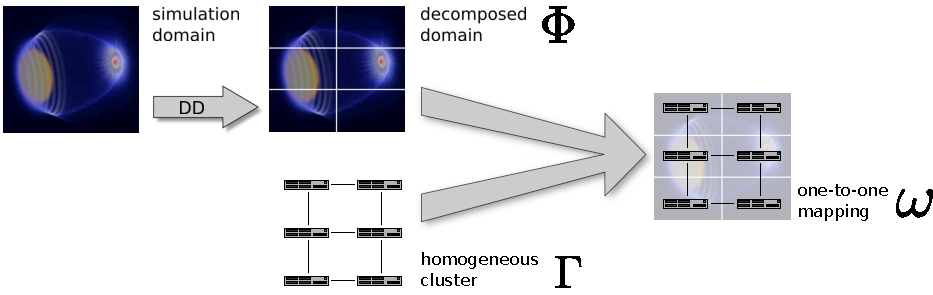
\includegraphics[width=\textwidth]{graphics/30_domain_decomposition}
  \caption{The simulation domain is decomposed in subdomains. These subdomains
    are mapped one-to-one onto the homogeneous cluster.}
  \label{fig:domain_decomposition}
\end{figure}

\noindent For most simulations executed on cluster systems is this approach
state of the art.  This approach works, as long as both hardware and
simulation stay in this fixed relationship. Thus, there is no change
necessary as long as a simulation will always be executed on the same
cluster, with the same network topology, and the same algorithms
describing the simulation model.

However, it is not possible to map all modern simulations in this
model of a homogeneous world. Some simulation applications have
horizontal and vertical heterogeneous behavior. In horizontal
direction, the workload of subdomains can vary during the time of
simulation. The simulation runs into an unbalanced state of workload
distribution. Figure \ref{fig:load_balancing} shows the workload
distribution of the simulation domain through a heat map. The workload
distribution changes after a certain time $\Delta t$. Therefore, the
simulation is decomposed again an mapped with a new $\omega$ to the
hardware topology.

\begin{figure}[H]
  \centering 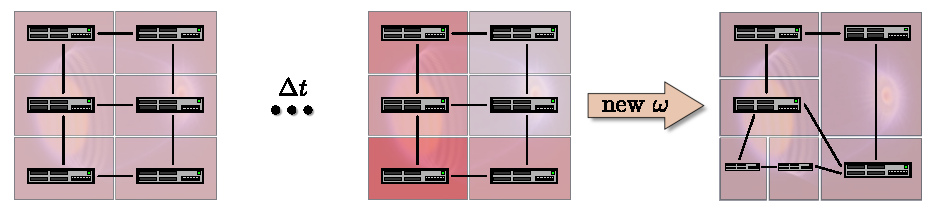
\includegraphics[width=\textwidth]{graphics/30_load_balancing}
  \caption{Vertical heterogeneity by unbalanced load distribution
    after a time $\Delta t$ presented through a heat map.  The
    simulation domain is decomposed again and mapped with a new
    $\omega$ to the hardware topology.}
  \label{fig:load_balancing}
\end{figure}

\noindent Furthermore, implies a failure of a node the termination of subdomain
calculations on this node. The simulation can be continued if the
subdomain of the failed node can be mapped to another node. Figure \ref{fig:resilience}
shows the failure of a node during simulation after a time $\Delta t$.
The subdomain of the failed node is mapped with a new $\omega$.

\begin{figure}[H]
  \centering 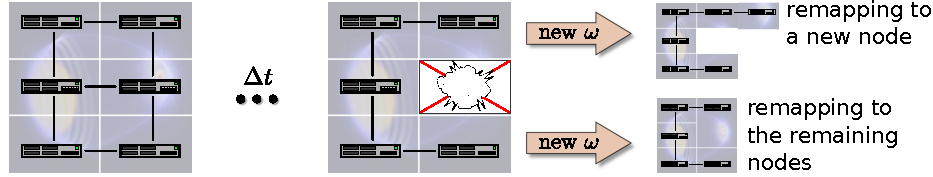
\includegraphics[width=\textwidth]{graphics/30_resilience}
  \caption{ }
  \label{fig:resilience}
\end{figure}

Even though there is an optimal mapping $\omega$ for a time step
$t_0$, it does not imply that the same mapping is optimal for time
step $t_1$.  Thus, a simulation behaves horizontal heterogeneous if
$\omega(t_0) \neq \omega(t_1)$.

In vertical
direction, multiscale effects, each representing a specific algorithm
of the simulation, which leads to varying communication topologies between
subdomains. Every communication topology usually requires
sophisticated, time consuming programming. 


That unbalanced
state does neither saturates all available computing resources nor does it
minimize the overall simulation time. Additionally, a globally
increased workload might require a redistribution of the simulation
domain onto the computing nodes at run-time.

Not only the simulation can be heterogeneous, but also the cluster
hardware on which the simulation is executed
(Section~\ref{sec:accel}): vertical cluster heterogeneity describes
the usage of multisocket, multicore, and or additional accelerator
hardware in cluster nodes, where each of these compute devices has its
own hierarchical memory structure. This hardware needs to be
programmed with caution and knowledge about the device to achieve
maximal performance.  Also, horizontal differences of cluster nodes
are possible. For example, a cluster can consist of varying node types
for different tasks in the simulation application. Therefore, the
simulation domain can not be mapped one-to-one on such a cluster
configuration, but rather the mapping should be configurable
explicitly. Figure~\ref{fig:heterogeneous_cluster_node} shows, in
contrast to an implicit one-to-one mapping, such an explicit mapping from the
simulation domain onto a heterogeneous computing system. This example
computing systems shows several device hierarchies. A single node has
two sockets each equipped with a multicore CPU and each CPU has access
to a pair of accelerator devices.

\begin{figure}[H]
  \centering
  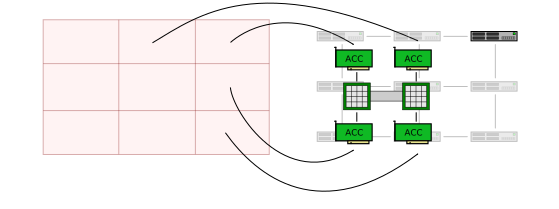
\includegraphics[width=\textwidth]{graphics/30_heterogeneous_cluster_node}
  \caption{Explicit mapping of subdomains onto a node of a
    heterogeneous and hierarchical computing system. The illustrated
    node has two sockets each equipped with a multicore CPU and each
    CPU has access to a pair of accelerator devices.}
  \label{fig:heterogeneous_cluster_node}
\end{figure}

A real world example for such heterogeneous behavior of simulations is
the PIConGPU simulation (Section \ref{sec:picongpu}). While magnetic
and electric fields only influence their directly neighboring fields,
particles interact globally with each other. The former necessitates
next neighbor and the latter all-to-all communication
algorithms. Furthermore, during simulation, particles can move to other
subdomains, which leads to an unbalanced distribution of particles
over the entire simulation domain.

On the hardware side, PIConGPU is developed for the execution on
cluster systems with NVIDIA accelerator hardware.  CPUs are
responsible for data offloading and communication over the network,
some of the available accelerators compute the interaction of fields
and particles, while others generate a visualization of the simulated
data. Thus, vertical and horizontal heterogeneity, both in simulation
domains and on the hardware cluster, are already present in real world
simulation applications.

Nowadays, state of the art communication libraries can not be adapted
to the needs of modern simulation applications.  Therefore, there
should be an intermediate layer between simulation application and the
software stack of the cluster. This layer should allow for an explicit
mapping of the simulation domain onto the communication library, while
the communication library should be easily exchangeable. With such a
setup, the mapping can be adjusted to heterogeneous behavior of
simulation application and cluster hardware.  As an added benefit,
this layer can be used to address problems like load balancing and
fault tolerance. However, both of these problems will not be addressed
by this system directly. Instead it should be possible to build an
application that supports both fault tolerance and load balancing
based on this system.

To address these issues, an approach for a flexible mapping of
communication processes onto arbitrary communication libraries was
designed. This design will be presented in the following
sections. At first, the requirements for such a system are
discussed. It is followed by a description of the overall design and
finally the design of each component is discussed in detail.
%%%%%%%%%%%%%%%%%%%%%%%%%%%%%%%%%%%%%%%%%%%%%%%%%%%%%%%%%%%%%%%%%%%%%%%%%%%%%%%%
%                                                                              %
% ANALYSIS OF PIConGPU CODE                                                    %
%                                                                              %
%%%%%%%%%%%%%%%%%%%%%%%%%%%%%%%%%%%%%%%%%%%%%%%%%%%%%%%%%%%%%%%%%%%%%%%%%%%%%%%%
%% \section{Analyzing the PIConGPU Application}
%% \label{sec:picongpu_analysis}

%% The analysis of the PIConGPU source code and modeled simulation domain
%% plays as significant role in the design of the developed system.

%% The PIConGPU domain is divided into a three-dimensional grid of cells.
%% Each cells computes effects of particles and fields. Fields interact
%% with fields of neighboring cells. Therefore, is a communication with
%% neighboring cells necessary. Particles interact with all other
%% particles. Therefore, is a all-to-all communication with all other
%% cells necessary.

%% PIConGPU uses plain MPI as communication back end. Some MPI calls
%% are covered by a communicator class, some are used directly in
%% the source code. Data exchange of neighboring cells is performed
%% by non-blocking point-to-point operations. Certain algorithms
%% make use of collective operations to collect data among a particular
%% amount of cells.


%%%%%%%%%%%%%%%%%%%%%%%%%%%%%%%%%%%%%%%%%%%%%%%%%%%%%%%%%%%%%%%%%%%%%%%%%%%%%%%%
%                                                                              %
% REQUIREMENTS                                                                 %
%                                                                              %
%%%%%%%%%%%%%%%%%%%%%%%%%%%%%%%%%%%%%%%%%%%%%%%%%%%%%%%%%%%%%%%%%%%%%%%%%%%%%%%%
% Checked
\section{Requirements}
\label{sec:requirements}

The previous Section~\ref{sec:motivation} described the state of the
art of simulations on cluster systems and gave a motivation to solve
the problems of modern simulations.
%% Furthermore, analyzed
%% Section~\ref{sec:picongpu_analysis} the PIConGPU application with
%% respect to its needs for a enhanced communication approach.
It was determined that an intermediate layer between application and
communication library is required.  This layer should offer the
possibility to describe the communication processes of the simulation
in a very general manner.  The construction of this intermediate layer
involves three steps.  First, existing communication libraries should
be abstracted by a general communication interface. Thus,
communication is not restrict to a single communication library and,
therefore, incraeses the simulations portability.  Second, the
communication topology of the simulation should be modeled explicitly,
so that the modeled communication topology can be mapped explicitly
onto an communication abstraction layer.  Third, the combination of
modeled communication topology and the abstraction from communication
libraries form an approach to communicate virtually on basis of the
described communication topology.  In summary, the discussion on the
intermediate layer result in the following three requirements of the
referred problems of modern simulations:

\begin{enumerate}
\item Abstract data exchange method
\item Modeling of the communication topology
\item Mapping of communiation topology onto the abstract communication interface
%\item Virtual data exchange method 
\end{enumerate}



%%%%%%%%%%%%%%%%%%%%%%%%%%%%%%%%%%%%%%%%%%%%%%%%%%%%%%%%%%%%%%%%%%%%%%%%%%%%%%%%
%                                                                              %
% THE SYSTEM                                                                   %
%                                                                              %
%%%%%%%%%%%%%%%%%%%%%%%%%%%%%%%%%%%%%%%%%%%%%%%%%%%%%%%%%%%%%%%%%%%%%%%%%%%%%%%%
% Checked 
\section{Design Overview}

Physical networks such as Ethernet, Infiniband or Myrinet are the
foundation of common communication libraries such as MPI
(Section~\ref{sec:mpi}).  State of the art simulation applications are
usually implemented directly on these existing communication
libraries. The developed system introduces an intermediate layer
between application and communication library. This layer fulfills all
requirements set up in Section~\ref{sec:requirements}. Figure
\ref{fig:design} shows the components of this intermediate layer and
which requirement they fulfill.  On top of the existing communication
libraries the communication abstraction Layer (CAL) uses library
specific adapters to provide a general interface for upper layer.  A
graph is used to model the communication topology of the simulation
domain and a graph-based virtual overlay network maps this graph onto
the hardware topology of the communication abstraction layer.

\begin{figure}[H]
  \centering 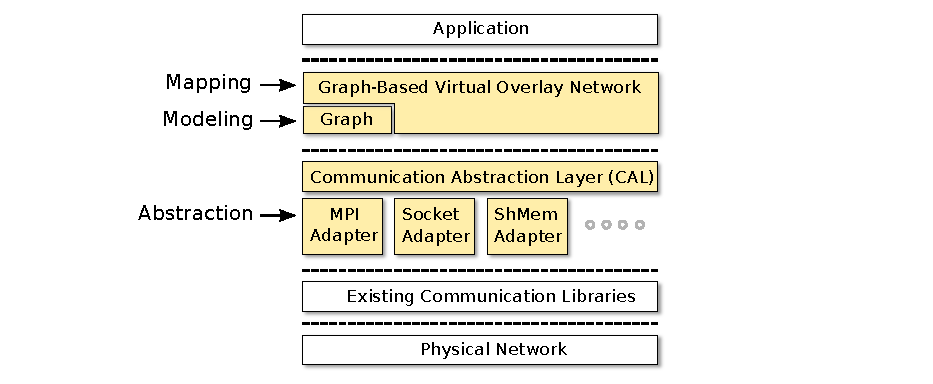
\includegraphics[width=\textwidth]{graphics/30_design}
  \caption{Design of the developed system in layers. An intermediate
    layer between application and communication library is introduced.
    This layer provides the communication abstraction layer (CAL), the
    graph description of the communication topology, and the
    graph-based virtual overlay network (GVON). These components
    fulfill the discussed requirements in
    Section~\ref{sec:requirements}.}
  \label{fig:design}
\end{figure}

\noindent The following sections discuss each component in detail:
Section~\ref{sec:comm_abstraction} presents the CAL;
Section~\ref{sec:graph} explains the graph interface;
Section~\ref{sec:gvon} follows up with the GVON.  Component interfaces
will be described in some cases by pseudo-code which is related to the
C++ programming language. It is assumed, that the reader has a basic
knowledge of programming and function interfaces.

%%%%%%%%%%%%%%%%%%%%%%%%%%%%%%%%%%%%%%%%%%%%%%%%%%%%%%%%%%%%%%%%%%%%%%%%%%%%%%%%
%                                                                              %
% COMMUNICATION ABSTRACTION LAYER                                              %
%                                                                              %
%%%%%%%%%%%%%%%%%%%%%%%%%%%%%%%%%%%%%%%%%%%%%%%%%%%%%%%%%%%%%%%%%%%%%%%%%%%%%%%%
% Checked
\section{Abstraction from Existing Communication Libraries}
\label{sec:comm_abstraction}

% Motivation for communication abstraction
Simulation applications can be interconnected by a vast variety of
communication libraries. Most simulations utilize exactly one possible
libarary, but this restricts the simulation to computing systems which
only support the selected library (Figure
\ref{fig:design_state_of_the_art}).

\begin{figure}[H]
  \centering 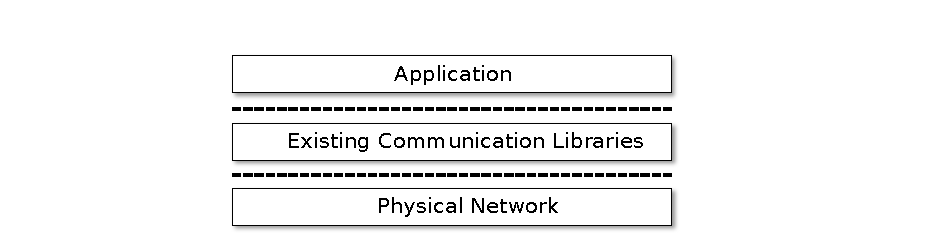
\includegraphics[width=\textwidth]{graphics/30_design_state_of_the_art}
  \caption{The simulation application is implemented directly on top
    of a communication library.}
  \label{fig:design_state_of_the_art}
\end{figure}

Assuming, that a simulation is distributed on a several computers and uses a
communication library based on TCP/IP sockets. The execution of this
simulation on a single machine is an interesting use case for
testing. It results in no problem when the simulation is executed on
this local machine and communicates locally by sockets.  But, it might
be more efficient to use shared memory to exchange data between
subdomains, instead of TCP/IP messages.

However, exchanging the communication interface in the example above,
usually requires a lot of reprogramming of the communication logic.
Therefore, it is not a sufficient solution for the problem.  Rather,
varying communication libraries should by addressable by the same
communication interface to make the application portable for varying
computing environments. Although, there are existing standards for
communication in cluster systems, the world of computer science is
subject to constant change.  The possibility to exchange the
underlying layer without changing the interface to this layer is a
precondition for future applications in distributed computing.  Thus,
the abstraction from this existing communication libraries is a
fundamental property for a portable application.

The challenge is to provide a very general interface, that provides
the possibility to address varying communication libraries through it.
This interface should be as common as possible and should be easily
deployable into existing applications by replacing the actual
communication library without changing the fundamental understanding
of the way to communicate within this application. The following
section describes the design of such an abstract communication
interface.


%%%%%%%%%%%%%%%%%%%%%%%%%%%%%%%%%%%%%%%%%%%%%%%%%%%%%%%%%%%%%%%%%%%%%%%%%%%%%%%%
%                                                                              %
% CAL                                                                          %
%                                                                              %
%%%%%%%%%%%%%%%%%%%%%%%%%%%%%%%%%%%%%%%%%%%%%%%%%%%%%%%%%%%%%%%%%%%%%%%%%%%%%%%%
% Checked
\subsection{Communication Abstraction Layer}
\label{sec:cal}

The \textit{Communication Abstraction Layer}, short \textit{CAL}, is a
general communication interface on top of an existing communication
library. The libraries are accessible through adapters, which makes it
possible to access varying communication libraries. By exchanging the
adapter, the application based on the interface can be ported to
varying communication libraries without changing interface function
calls. The CAL is configured with a certain adapter at compile
time. Thus, by using this flexible approach, no run-time overhead
should occur. The evaluation of the developed system in
Section~\ref{sec:evaluation} will show the run-time overhead with
respect to MPI.

The CAL provides an abstract interface for common communication
operations. The adapter needs to implement the interface demanded by
the CAL.  The Communication operations are performed by existing
communication libraries wrapped by an adapter.

Instances participating on communication in general are called peers
in the following.  The interface of the CAL provides basic
point-to-point communication operations (Section~\ref{sec:des:p2p}),
collective operations (Section~\ref{sec:cal_collective}) and
operations for grouping of peers (Section~\ref{sec:cal_context}).
Figure \ref{fig:cal} shows the communication abstraction layer on top
of existing communication libraries.  The CAL with a specific adapter
could already replace a certain communication library in a simulation
application, but it is not meant to be the level of abstraction the
simulation programmer will interact with. The design of further layers
of abstraction will be discussed in Sections \ref{sec:graph} and
\ref{sec:gvon}.

\begin{figure}[H]
  \centering
  
\includegraphics[width=\textwidth]{graphics/30_design_cal}
  \caption{Communication Abstraction Layer (CAL) on top of existing
    communication layers. Varying communication libraries can be
    addressed through the CAL interface, when an according adapter for
    this library is implemented.}
  \label{fig:cal}
\end{figure}


\noindent Using the CAL instead of a concrete communication library has
the advantage, that only the adapter needs to be replaced when
changing the communication environment, for example when migrating
to another compute architecture. Although, the application has
to be recompiled, the CAL interface stays the same.


%The CAL has the requirement, that peers need to be connected directly
%by the network of the adapter.
%Peers have to be connected directly by the network of the
%adapter.
%Because, It is not planed that the CAL provides routing
%abilities.
%No routing makes it impossible to forward data between
%different adapters of the CAL. Thus a specific CAL only provides a
%single adapter.
%But several CALs can be used with different adapters
%to communicate on several networks.
%In such a scenario a kind of
%routing can be implemented on top of the CAL by the system
%user.
%Therefore, the design was first pushed forward in the direction
%of a single adapter design and considerations regard to a multiple
%adapter design is left open for future work.


%%%%%%%%%%%%%%%%%%%%%%%%%%%%%%%%%%%%%%%%%%%%%%%%%%%%%%%%%%%%%%%%%%%%%%%%%%%%%%%%
%                                                                              %
% ADDRESSING OF PEERS                                                          %
%                                                                              %
%%%%%%%%%%%%%%%%%%%%%%%%%%%%%%%%%%%%%%%%%%%%%%%%%%%%%%%%%%%%%%%%%%%%%%%%%%%%%%%%
% Checked
\subsection{Addressing of Peers}
% CAL virtual addressing
Each communication library provides a particular approach to address
peers. Internet socket based systems
address their peers by IP addresses, MPI based systems address their
processes by ranks, and shared memory based systems are utilizing
memory addresses.  These diverse approaches to address peers in a
network need to be translated to an unified address space to provide a
single interface for the CAL user.  Therefore, the CAL provides a
virtual address, short \emph{vAddr}, which is an unique identifier for
its peer. Based on this virtual address, peers are able to address
each other through the CAL interface.

The translation of virtual addresses to the adapter specific real
address is resolved by the adapter itself. Thus, the adapter defines
how the participants of its network are mapped onto the given virtual
address space of the CAL. This mapping is hidden from the CAL, so that
the CAL only needs to handle virtual addresses and the adapter handles
its particular address space.

%%%%%%%%%%%%%%%%%%%%%%%%%%%%%%%%%%%%%%%%%%%%%%%%%%%%%%%%%%%%%%%%%%%%%%%%%%%%%%%%
%                                                                              %
% CAL INTERFACE                                                                %
%                                                                              %
%%%%%%%%%%%%%%%%%%%%%%%%%%%%%%%%%%%%%%%%%%%%%%%%%%%%%%%%%%%%%%%%%%%%%%%%%%%%%%%%
% Peer2Peer Operations
\subsection{Point-to-Point Communication Methods}
\label{sec:des:p2p}

In the first place the CAL provides point-to-point communication
methods. These are basic communication methods to exchange abitrary
data between two peers, which are available in blocking and
non-blocking variants.

A non-blocking communication method returns an \emph{event} object that represents
the state of the executed communication method. The state
of the \emph{event}t is either \emph{ready} or \emph{not ready}. An
\emph{event} provides functions to request the current state and 
to  wait until the method has finished. The CAL only provides the
event interface. Adapters implement the  event interface for their
particular communication library since each libary treats non-blocking
communication differently \cite{ref:mpi_specification,ref:boost_asio}.

A point-to-point communication method is called with a triplet of
arguments: the virtual address of sender or receiver, the message
description tag, and the actual data object to exchange.  The design
of this interface was influenced by existing communication libraries
that all share a common interface \cite{ref:boost_mpi, ref:boost_asio,
  ref:zmq}. The message description tag is the header of the
message. It helps to distinguish between messages of the same sending
peer.  The data object must provide methods to retrieve the data
pointer and the size of the data. The data pointer must point to a
contiguous memory area. The following lists the point-to-point
communication methods of the CAL interface:

\begin{itemize}
  %% \item  \textbf{void send(destinationVAddr, tag, data);}
  %% \item  \textbf{void recv(sourceVAddr, tag, data);}
  %% \item  \textbf{Event asyncSend(destinationVAddr, tag, data);}
  %% \item  \textbf{Event asyncSecv(sourceVAddr, tag, data);}

  \item  void \textbf{send }(destinationVAddr, tag, data)
  \item  void \textbf{recv }(sourceVAddr, tag, data)
  \item  Event \textbf{asyncSend }(destinationVAddr, tag, data)
  \item  Event \textbf{asyncSecv }(sourceVAddr, tag, data)

\end{itemize}

%%%%%%%%%%%%%%%%%%%%%%%%%%%%%%%%%%%%%%%%%%%%%%%%%%%%%%%%%%%%%%%%%%%%%%%%%%%%%%%%
%                                                                              %
% CONTEXT                                                                      %
%                                                                              %
%%%%%%%%%%%%%%%%%%%%%%%%%%%%%%%%%%%%%%%%%%%%%%%%%%%%%%%%%%%%%%%%%%%%%%%%%%%%%%%%
% Checked
\subsection{Grouping of peers}
\label{sec:cal_context}
Besides the communication methods,grouping of peers is the most
important function the CAL provides through its interface.  By
default, all peers of the CAL are members of the global group of peers.
A group of peers will be called \textit{context}. Accordingly, the
global group of peers is called \emph{global context}. A context is valid for
all contained peers. In turn, it is invalid for all peers not
contained.

A context stores the set of virtual addresses of its members , the
number of members, and whether the context is valid for a particular
peer. It is the base for communication algorithms with more than two
participating peers.
% These algorithm are introduced as collective operations (Section \ref{sec:cal_collective}).

The CAL always provides the global context from which a peer can
retrieve its global virtual address. A new context can be created from
a subset of peers of an already existing context. Hence, a new context
can be created according to the requirements of the communication
algorithm. This new context provides its own virtual address space,
thus, the virtual address of a peer is context dependent.

Each adapter can handle contexts differently. The CAL only
defines the context interface, but each adapter needs to implement the
context interface for its particular communication
library. The adapter must respect that a virtual address
is context dependent. Therefore, the mapping of a virtual address to a
real address has to be adapted to the currently used context.

%%%%%%%%%%%%%%%%%%%%%%%%%%%%%%%%%%%%%%%%%%%%%%%%%%%%%%%%%%%%%%%%%%%%%%%%%%%%%%%%
%                                                                              %
% COLLECTIVE OPERATIONS                                                        %
%                                                                              %
%%%%%%%%%%%%%%%%%%%%%%%%%%%%%%%%%%%%%%%%%%%%%%%%%%%%%%%%%%%%%%%%%%%%%%%%%%%%%%%%
% Checked
\subsection{Collective Operations}
\label{sec:cal_collective}
A \textit{collective operation}, short \textit{collective}, is a
communication pattern that is executed simultaneously by all peers of
a context. For example are collectives utilized to collect,
share and reduce data.  Each collective can be implemented by a
sequence of peer to peer operations, but communication libraries,
especially the ones for high performance calculations such as MPI
(Section~\ref{sec:mpi}), often provide optimized collective support.

A collective is always executed with respect to a context and the
result is either received by a single peer, the root, or by all peers.
While a large number of collectives is known to the parallel
computation commmunity, the CAL only provides the most common ones
with respect to the analysis of the PIConGPU source code
(Section~\ref{sec:picongpu}).  However, other collectives are
implementable in future work. The following is lists a subset of the
provided collective operations of the CAL and their description:


\begin{itemize}
\item  void \textbf{gather} (rootVAddr, context, send, recv)\\
  Collection of data elements from every peer in the context. Each
  peer contributes the same number of data elements. The collected
  data is received by the root peer.

%\item void \textbf{allGather} (context, send, recv)\\
%  The same as gather(), but all peers of the context receive the data.

\item  void \textbf{scatter} (rootVAddr, context, send, recv)\\
  Distribution of data elements from the root peer to all other peers of
  the context. The data is divided into chunks of same
  size, depending on the number of peers. One chunk is send to each peer.

%\item  void \textbf{allScatter} ( context, send, recv)
%  The same as scatter(), but all peers of the context receive the same.

\item  void \textbf{reduce} (root, context, binOperation, send, recv)\\
  Reduction of data elements from every peer of a context
  by a binary function that takes arguments of an arbitrary type
  and returns a values of the same type.

%\item  void \textbf{allReduce}  (context, operation, send, recv)\\
%  The same as reduce(), but all peers of the context receive the
%  result of the reduction.

\item  void \textbf{broadcast} (root, context, data)\\
  Distributes data elements from the root peer to all other peers of
  the context. Every peer receives the same data elements.

\item  void \textbf{syncronize} (context)\\
  This operation synchronizes the control flow of all peers of the
  context.

\item  void \textbf{createContext} (peers, context)\\ 
  Creation of a new context from a subset of peers of an already
  present context.

\end{itemize}

\noindent All peers of the listed collectives send or receive the same
number of elements.  But some algorithms require an exchange of
varying number of elements. Therefore, the collectives gather and
scatter are also available in a variant with varying number of
elements per peer. These collectives get an additional receive count
argument, that describes how many data elements each peer has
contributed to the collective. Furthermore are the operations gather,
scatter, and reduce available in an all receive variant. All senders
of the collective will receive the collective result. Therefore, the
specification of a root peer can be omitted in for these variants.


%%%%%%%%%%%%%%%%%%%%%%%%%%%%%%%%%%%%%%%%%%%%%%%%%%%%%%%%%%%%%%%%%%%%%%%%%%%%%%%%
%                                                                              %
% GRAPH                                                                        %
%                                                                              %
%%%%%%%%%%%%%%%%%%%%%%%%%%%%%%%%%%%%%%%%%%%%%%%%%%%%%%%%%%%%%%%%%%%%%%%%%%%%%%%%
% Checked
\section{Modeling of the Application Domain by a Graph}
\label{sec:graph}
A simulation model is usually implemented through a particular
algorithm in the simulation application.  Porting this algorithm onto
a parallel computing system requires a decomposition
(Section~\ref{sec:domain_decomposition}) of the simulation domain into
a set of subdomains.  Communication is necessary if these subdomains
need to interact with each other.  Whereby, the communication topology
of the simulation is determined by the algorithm.

%% Communication topologies are often implemented in a implicit and
%% static fashion. A change of the simulation algorithm needs to be translated
%% into a change of the corresponding communication patterns, which can
%% be quiet costly. Furthermore, would a reutilization of already modeled
%% communication topologies reduce implementation effort of
%% implementations of future simulations.

%% \paragraph*{}
%% A more elegant approach is the explicit modeling of relationships
%% between the subdomains. Therefore, the communication topology of the
%% simulation.

The most general method to model a topology is a
\emph{graph}~\cite{ref:graph}. Furthermore, the explicit modeling of
the communication topology by a graph has the advantage that the reuse
of this topology reduces the implementation effort for future
simulation applications.  A graph consists of vertices and
edges. Edges are described as a pairs of vertices.

%So to speak, a
%graph represents a set of objects, where some of these objects are
%connected by links.

% directed cycle multi graph
Vertices of the graph used in further descriptions are connected by
directed edges.  Loops and multiple edges between two vertices are
allowed (Figure~\ref{fig:graph}). Together this results in a directed
multigraph with loops, which is called a quiver \cite{ref:quiver}.

\begin{figure}[H]
  \centering 
\includegraphics[width=\textwidth]{graphics/30_graph}
  \caption{The graph interface describes quivers. It is shown a
    directed cycle multi graph with four vertices. Graphs can be
    used to describe the communication topology of domain decomposed
    applications.}
  \label{fig:graph}
\end{figure}

\noindent Changing the simulation algorithm implies a different
communication topology and in turn implies a different graph. The
graph has the advantage, that the communication topology is
modeled explicitly. It is not necessary to rewrite the simulation
application as long as the application is based on the topology
information provided by the graph. Thus, communication processes can
by implemented on top of the graph description. The presented graph
should be addressable by the following interface:

\begin{itemize}
  \item VertexList \textbf{getVertices} ()\\
    Returns the list of all vertices of the graph.
    
  \item  Vertex \textbf{getVertex} (index)\\
    Returns a particular vertex by vertex \textit{index}.

  \item  VertexList \textbf{getAdjacentVertices} (vertex)\\
    Returns a list of all adjacent vertices of \textit{vertex}.

  \item  EdgeList \textbf{getOutEdges} (vertex)\\
    Returns a list of all outgoing edges from the \textit{vertex}
    paired with their target vertex.

  \item  EdgeList \textbf{getInEdges} (vertex)\\
    Return a list of all incoming edges to the \textit{vertex}
    paired with their source vertex.

  \item  Graph \textbf{createSubGraph} (vertices)\\
    Returns a subgraph, that only contains the defined
    \textit{vertices} from the supergraph.
\end{itemize}

%%%%%%%%%%%%%%%%%%%%%%%%%%%%%%%%%%%%%%%%%%%%%%%%%%%%%%%%%%%%%%%%%%%%%%%%%%%%%%%%
%                                                                              %
% GRAPH PROPERTIES                                                             %
%                                                                              %
%%%%%%%%%%%%%%%%%%%%%%%%%%%%%%%%%%%%%%%%%%%%%%%%%%%%%%%%%%%%%%%%%%%%%%%%%%%%%%%%
% Checked
\subsection{Properties}
A graph viewed in isolation is only a representation of connected
vertices, not providing further information. Interpreting the graph as
a C++ object container offers the possibility to insert objects into the graphs
vertices and edges.

An object that resides in this containers will be called property and
is introduced as a concept to annotate a graph. A property usually
provides subdomain information and can be bound to vertices and edges
(Figure \ref{fig:property}). Each vertex and edge of the same graph
share the same type of property. A graph annotated with
properties is significantly more meaningful and therefore helps to
keep the connection between the simulation domain and communication
topology.

\begin{figure}[H]
  \centering 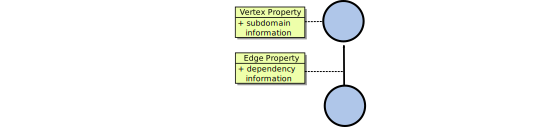
\includegraphics[width=\textwidth]{graphics/30_property}
  \caption{A graph annotated with both vertex and edge properties. The vertex
    property primarily describes a subdomain. The edge property
    describes the dependencies between subdomains.}
  \label{fig:property}
\end{figure}

\noindent The field of application of properties can by diverse. It highly
depends on the graph and its area of utilization.  A property can also
be used to create a connection between a pair of graphs, resulting a
hierarchical description.



%%%%%%%%%%%%%%%%%%%%%%%%%%%%%%%%%%%%%%%%%%%%%%%%%%%%%%%%%%%%%%%%%%%%%%%%%%%%%%%%
%                                                                              %
% MODELING GAME OF LIFE AS A GRAPH                                             %
%                                                                              %
%%%%%%%%%%%%%%%%%%%%%%%%%%%%%%%%%%%%%%%%%%%%%%%%%%%%%%%%%%%%%%%%%%%%%%%%%%%%%%%%
% Checked
\subsection{Modeling Game of Life as a Graph}
\label{sec:gol}
To give an example on how to model a specific simulation application,
Figure~\ref{fig:gol_modeling} shows the modeling of the Game of Life
(GoL)~\cite{ref:gol} domain by a graph. The GoL simulates the evolution of
a set of cells for an arbitrary amount of time steps. The cells are
arranged in a two-dimensional grid (Figure \ref{fig:gol_simulation}).
A cell has a state which is either alive or not alive and the state of
the next time step is calculated by rules.  The common set of rules
determines the state of a cell for the next time step using current
state information of the neighboring cells.  Assume the rule: ``a dead
cell with exactly three living cells in the neighborhood will be reborn on
the next time step'' is the only existing rule in further descriptions
of GoL.  Nevertheless, a GoL simulation can consist of a arbitrary set
of rules.

\begin{figure}[H]
  \centering 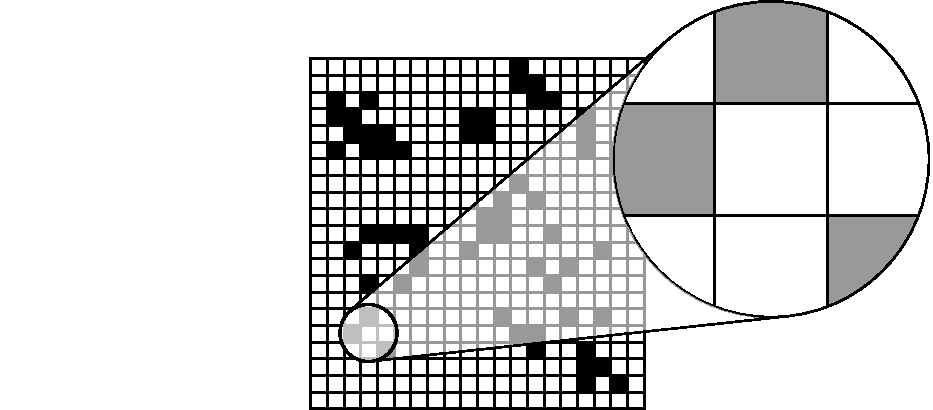
\includegraphics[width=\textwidth]{graphics/30_gol_simulation}
  \caption{Image detail of a GoL domain showing 9 neighboring cells. The GoL
    domain is a rectangular grid of cells.  Cells have a state, while
    living cells are colored dark, dead cells are white. The state of
    a cell for the next time step is determined by a set of rules.}
  \label{fig:gol_simulation}
\end{figure}

\noindent The GoL simulation is modeled as follows:
every cell is represented by a vertex and neighboring cells are
connected by an edge.  Each vertex has the property \emph{Cell}, which
contains the state of the cell. Figure \ref{fig:gol_modeling} shows a
visualized image detail of the modeled GoL domain. To determine the next
state of a cell, the number of living adjacent cells have to be counted. The cell
will be alive on the next time step, if exactly three adjacent cells
are alive.


\begin{figure}[H]
  \centering 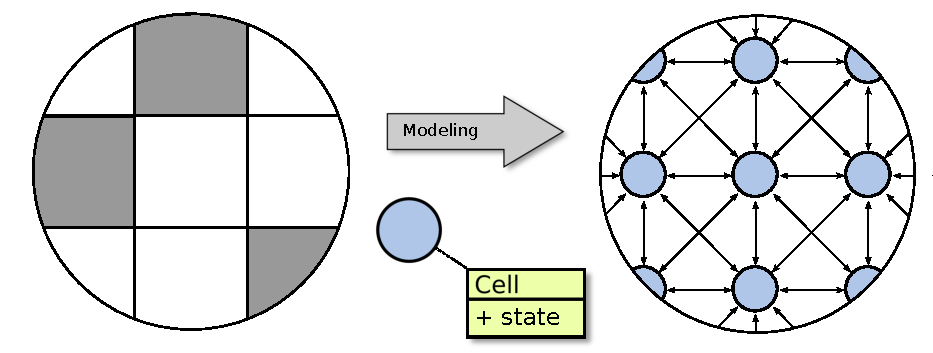
\includegraphics[width=\textwidth]{graphics/30_gol_modeling}
  \caption{Image detail of a Game of Life domain (on the left) was modeled
    as a graph (on the right). Each Vertex is described by the vertex
    property \emph{Cell}, containing the state information of the cell.}
  \label{fig:gol_modeling}
\end{figure}

\noindent The rule is now changed slightly: a cell is alive on the next time
step when at least one diagonal neighbor is alive.  A changed rule
 implies a change in the GoL algorithm.  This changes the GoL
communication topology and therefore the modeled
graph. Figure~\ref{fig:gol_modeling_changed} models the GoL domain
with the changed rule. Vertices are connected with its diagonal
located vertices. Nevertheless, to determine the next state of a cell
the number of living adjacent cells have to be counted.

\begin{figure}[H]
  \centering 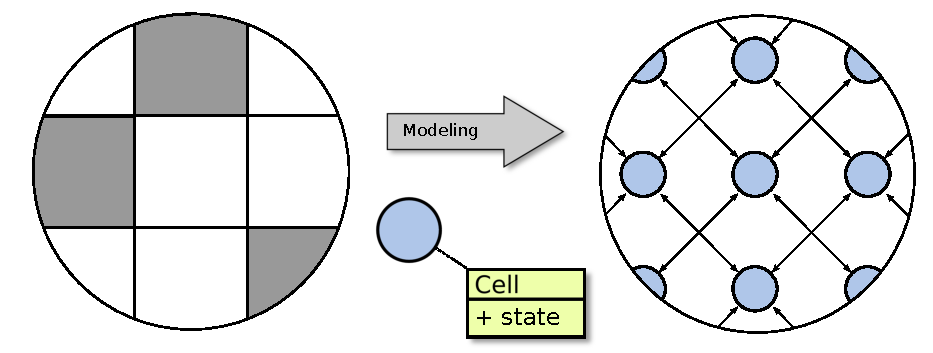
\includegraphics[width=\textwidth]{graphics/30_gol_modeling_changed}
  \caption{Image detail of a Game of Life domain (on the left)
    modeled with a different rule (on the right. Only diagonal located
    vertices are connected.}
  \label{fig:gol_modeling_changed}
\end{figure}


%%%%%%%%%%%%%%%%%%%%%%%%%%%%%%%%%%%%%%%%%%%%%%%%%%%%%%%%%%%%%%%%%%%%%%%%%%%%%%%%
%                                                                              %
% PARTITIONING THE GoL GRAPH                                                   %
%                                                                              %
%%%%%%%%%%%%%%%%%%%%%%%%%%%%%%%%%%%%%%%%%%%%%%%%%%%%%%%%%%%%%%%%%%%%%%%%%%%%%%%%
% Checked
\subsection{Partitioning the GoL Graph}
The graph in Figure~\ref{fig:gol_modeling} depicts the fine granular
model of the GoL domain, where each cell is represented by a vertex.
While it is the smallest possible domain decomposition, it might not
be very efficient when a single cell is calculated by a single
process. One process can compute considerably more cells.

Figure~\ref{fig:gol_bundle} shows the creation of a partitioned graph
by combining multiple vertices to partitions. Partitions are connected by edges when at least one cell at
the border of a partition is the neighbor cell of a border cell from
another partition.  The creation of a partioned graph  with a
minimum of connections is the topic of graph partitioning algorithms.

While the fine granular GoL graph represents the GoL cells in detail,
the partitioned graph represents dependencies of partitions. The GoL
graph and the partitioned graph can coexist and can be connected by their
properties. Thus, the properties of the partioned graph changed with
respect to the GoL graph, such that, partitions store the partitioned cells and
the partition connections refer to cells in neighboring partitions.

\begin{figure}[H]
  \centering 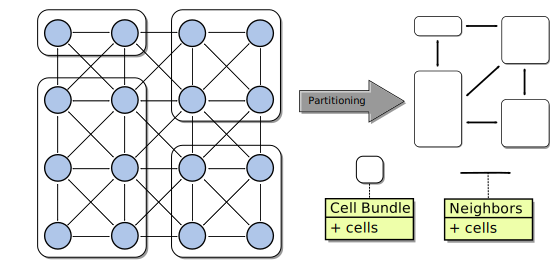
\includegraphics[width=\textwidth]{graphics/30_gol_bundle}
  \caption{The GoL graph is partitioned by combining multiple
    cells. The properties of the partioned graph have changed with
    respect to the GoL graph. The vertex property contains the cells
    of a partition, while the edge property contains information about
    border cells in neighboring partitions.}
  \label{fig:gol_bundle}
\end{figure}

\noindent The partitioned graph can be used as foundation to distribute GoL to
multiple nodes of a cluster. Each partition can be calculated by its own
process. The processes calculate a time step of their local GoL graph and
communicate the states of their border cells to adjacent bundles.

It has been introduced a different approach to model the Game of Life
domain. It used the same description language, the graph.  Fine
granular modeled domains can be partioned by common graph partition
algorithms to obtain more performance by clustering
vertices. A automated transformation from a graph description into a
more efficient graph description is an interesting topic, but not
covered by this work.


%%%%%%%%%%%%%%%%%%%%%%%%%%%%%%%%%%%%%%%%%%%%%%%%%%%%%%%%%%%%%%%%%%%%%%%%%%%%%%%%
%                                                                              %
% MODELING GAME OF LIFE AS A GRAPH                                             %
%                                                                              %
%%%%%%%%%%%%%%%%%%%%%%%%%%%%%%%%%%%%%%%%%%%%%%%%%%%%%%%%%%%%%%%%%%%%%%%%%%%%%%%%
% Checked
\subsection{Modeling a N-Body Simulation as a Graph}
\label{sec:design:nbody}
%% The second example to model a simulation application by a graph should provide
%% a completely different algorithm in respect to GoL. 

%% The N-body simulation, with a totally different algorithm in respect to GoL, was chosen as the
%% second example to model a simulation application by a graph.

The N-body simulation simulates particles in an two or three
dimensional space influenced by physical forces. The force considered
for this simulation is the gravity among each particle.  A particle is
described by its mass $m$, location $\overrightarrow{r}$ and velocity
$\overrightarrow{v}$.  The gravitational force between two particles
$i$ and $j$ can be calculated in a two-body model with the
gravitationlal constant $G$ by the Equation~\ref{eq:two_body_force}:

\begin{equation}
  \label{eq:two_body_force}
  \overrightarrow{F_{i,j}} = G  m_i  m_j \cdot \frac{\overrightarrow{r_j} - \overrightarrow{r_i}}{|\overrightarrow{r_j} - \overrightarrow{r_i}|^3}
\end{equation}

\noindent Equation~\ref{eq:n_body_force} describes the gravitational force of
particle $i$ to all other N-1 particles as the sum of each particular
force $\overrightarrow{F_{i,j}}$.

\begin{equation}
  \label{eq:n_body_force}
  \overrightarrow{F_{i,n}} = \sum_{j = 0 \atop j \neq i}^{N-1} \overrightarrow{F_{i,j}}
\end{equation}

\noindent Therefore, the force affecting particle $i$ is calculated by
considering velocity, mass and location of all other
particles. Modeling the particle dependencies results in an all-to-all
communication pattern with a complexity of
$O(N^2)$. Figure~\ref{fig:nbody_modeling} models the N-body domain
with $N = 6$ as a fully connected graph. Particles are represented as
pentagons in a two-dimensional space. The size of the particles
signals its mass and the arrow its velocity and direction.  In the
model, a vertex represents a particle and all particles are connected
via an edge. A vertex has the property \emph{Particle} that includes
the particle mass, location and velocity.

\begin{figure}[H]
  \centering 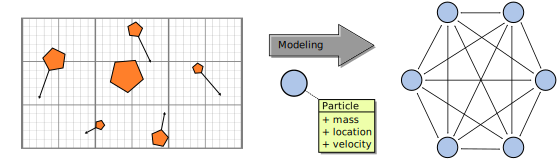
\includegraphics[width=\textwidth]{graphics/30_nbody_modeling}
  \caption{Modeling of an N-body domain with $N = 6$. A particle is
    represented by a vertex and each vertex is connected to all other
    vertices by edges.}
  \label{fig:nbody_modeling}
\end{figure}

\noindent A gravitational force on the particle $i$ results in a change of its velocity and
location after a fixed amount of time $t$. The following equations describe these
changes.

\begin{align}
  \label{eq:n_body_update}
  \overrightarrow{a} =&~ \frac{\overrightarrow{F_{i,n}}}{m}\\
  \overrightarrow{v} =&~ \overrightarrow{a} \cdot t + \overrightarrow{v_0}\\
  \overrightarrow{r} =&~ \frac{\overrightarrow{a}}{2} \cdot t^2 + \overrightarrow{v_0} \cdot t + \overrightarrow{r_0}
\end{align}


%%%%%%%%%%%%%%%%%%%%%%%%%%%%%%%%%%%%%%%%%%%%%%%%%%%%%%%%%%%%%%%%%%%%%%%%%%%%%%%%
%                                                                              %
% GRAPH-BASED VIRTUAL OVERLAY NETWORK (GVON)                                   %
%                                                                              %
%%%%%%%%%%%%%%%%%%%%%%%%%%%%%%%%%%%%%%%%%%%%%%%%%%%%%%%%%%%%%%%%%%%%%%%%%%%%%%%%
% Checked
\section{Graph-Based Virtual Overlay Network}
\label{sec:gvon}
The previous sections described the tools to communicate between
peers and to model a communication topology. The combination of these
tools establish a virtual communication layer within the simulation
domain. This layer is created by an explicit mapping of the
communication topology onto the CAL. Therefore, an application domain and its according
communication topology modeled by a graph can be used to perform
communication processes between subdomains.  This section introduces a
\emph{graph-based virtual overlay network}, short \emph{GVON},
that is based on the graphs and the CAL.

The graph does provide a simulation domain specific communication
topology.  It is used as a blueprint for the virtual network topology.
Communication operations are provided by the CAL as base for the
overlay network.  Figure \ref{fig:gvon} shows the GVON as a layer
between the graph and the CAL on one side and the application on the other
side.

\begin{figure}[H]
  \centering 
\includegraphics[width=\textwidth]{graphics/30_gvon}
  \caption{The graph-based virtual overlay network provides
    communication functionality based on the CAL, but uses the
    communication topology modeled by the introduced graph.}
  \label{fig:gvon}
\end{figure}

\noindent All peers that want to take part in the communication of the GVON need
to know exactly the same graph. In order to ensure that, the graph can be
constructed in parallel by all peers, loaded from the same file of a
distributed file system, or could even be delivered by a master
peer. Furthermore, peers need to use the same adapter configuring its
CAL, otherwise a communication is not possible.


%%%%%%%%%%%%%%%%%%%%%%%%%%%%%%%%%%%%%%%%%%%%%%%%%%%%%%%%%%%%%%%%%%%%%%%%%%%%%%%%
%                                                                              %
% GVON MAPPING                                                                 %
%                                                                              %
%%%%%%%%%%%%%%%%%%%%%%%%%%%%%%%%%%%%%%%%%%%%%%%%%%%%%%%%%%%%%%%%%%%%%%%%%%%%%%%%
% Checked
\subsection{Mapping of a Graph to the CAL}
\label{sec:mapping}
The connection between a graph and the CAL is a mapping of vertices
to peers, called the \emph{vertex map}.  A vertex map is valid for a
certain graph. Furthermore, the GVON provides a mapping of  graphs
to contexts (Section~\ref{sec:cal_context}), called the \emph{graph
  map}. This mapping is necessary since the GVON will also be used to
map collective operations on a graph to the CAL.  The vertex and
graph map are the basis for the mapping of communication processes
to the communication abstraction layer.  The mapping of vertices to
peers and graphs to contexts is a joint process of all peers that want to
participate in the communication based on a particular graph. This
mapping process is divided into two phases.

\subsubsection*{First Phase: Distribute}
The first phase distributes vertices of a graph to the peers, whereby
every vertex is assigned to a peer.  Figure~\ref{fig:gvon_mapping}
shows three peers and a graph of four vertices that are mapped to the
peers. It is possible that more than one vertex is mapped to a peer.
There are a variety of methods to distribute the vertices.  It could be
done randomized, round robin, consecutive, or dictated by
some master peer. The distribution behavior is defined by the user of
the GVON and might be object for further optimization.

\begin{figure}[H]
  \centering 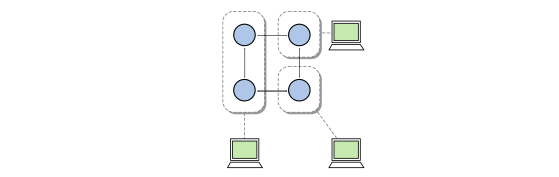
\includegraphics[width=\textwidth]{graphics/30_gvon_mapping}
  \caption{All vertices of a graph are distributed onto three
    peers. The vertices are not distributed evenly, thus, one peer is
    host for two vertices.}
  \label{fig:gvon_mapping}
\end{figure}

\subsubsection*{Second Phase: Announce}
In the second phase, the peers announce their mapped vertices to all
other peers.  A peer that announces vertices is called host and the
announced vertices are called hosted vertices.  Every host receives
from every other host a list of its hosted vertices.  This list is
used to update the vertex map and to create a new context only
including the hosts. The new context will be bounded to the graph of
the hosted vertices in the graph map.  A host is responsible for the
communication of its hosted vertices.  So to speak, it is also
possible that a host is responsible for all vertices of a graph and
communicates finally always with itself.  Depending on the used
adapter this might not even be a problem, since communication of a
host with itself can be performed in shared memory and does not
necessarily include network latency.


%%%%%%%%%%%%%%%%%%%%%%%%%%%%%%%%%%%%%%%%%%%%%%%%%%%%%%%%%%%%%%%%%%%%%%%%%%%%%%%%
%                                                                              %
% GVON COMMUNICATION                                                           %
%                                                                              %
%%%%%%%%%%%%%%%%%%%%%%%%%%%%%%%%%%%%%%%%%%%%%%%%%%%%%%%%%%%%%%%%%%%%%%%%%%%%%%%%
% Checked
\subsection{Communication within the GVON}
From the perspective of an overlay network, a vertex is interpreted as
a virtual peer, edges between adjacent vertices indicate that the
virtual peers are able to communicate with each other. An application,
implemented on top of the GVON, has the transparent view of exchanging
messages between vertices. The GVON is taking care, that the messages
reach the correct vertex host.  Finally, this is the level of
abstraction an application interacts with.

The GVON provides similar functionality like the presented
communication operations in the CAL in Section~\ref{sec:des:p2p}
and~\ref{sec:cal_collective}, but on graph basis. Therefore, both
point-to-point and collective operations are provided.

\subsubsection*{GVON Point-to-Point Methods}
A point-to-point operations within the GVON involves exchanging data
between adjacent vertices over an existing edge.  These operations
exist in blocking and non-blocking variants. While non-blocking
operations return an \emph{event} known from the CAL, nothing is returned by
blocking operations. The GVON provides the following interface for
point-to-point operations:

\begin{itemize}
  \item  void \textbf{send} (graph, destinationVertex, edge, data)
  \item  void \textbf{recv} (graph, sourceVertex, edge, data)
  \item  Event \textbf{asyncSend} ( graph, destinationVertex, edge, data)
  \item  Event \textbf{asyncRecv} ( graph, sourceVertex, edge, data)
\end{itemize}

\noindent The GVON has the task to resolv both the context of a graph
and the host of the source or destination vertex. This information are
queried from the vertex and graph map. When this information is
resolved the programm flow is handed over to the CAL. Finally, the CAL
is responsible for the data exchange.

% GVON collectives
\subsubsection*{GVON Collectives}
\label{sec:design:gvon_collectives}
Operations between all vertices of a graph can be performed as
collective operations (Section \ref{sec:cal_collective}).  The
collective has to be performed for all hosted vertices of a
host. Otherwise the overall execution of the operation is blocked by
the CAL. The operation is absolutely transparent for each vertex.  the
result of the collective is received by a root vertex or by all
vertices of the graph.

A collective operation is first executed locally for all hosted
vertices of a host. Afterwards, it is handled by the CAL and
transmitted to the receiver(s). Figure~\ref{fig:gvon_collective} shows
a gather operation on the same graph and mapping of
Figure~\ref{fig:gvon_mapping}. The gather operation collects the data
of hosted vertices of a host first locally and uses then the gather
operation provided by the CAL. A similar approach is used for the
reduce operation, whereby data is either collected or reduced locally
to a single value, depending on the commutativity of the reduce
operation.

The execution of the collective operation can be done sequentially or in
parallel. Both variants have their specific implementation and usage
specific problems. While sequential execution could lead to dead lock behavior
when a host forgets to execute the collective for at least one hosted vertex,
a parallel execution needs to ensure that the GVON is implemented in
a thread safe manner.

\begin{figure}[H]
  \centering 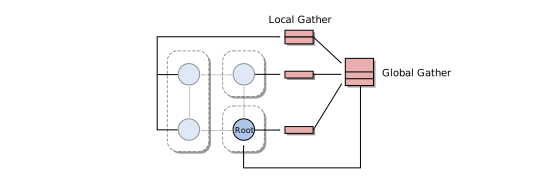
\includegraphics[width=\textwidth]{graphics/30_gvon_collective}
  \caption{Gather operation of the GVON. Data is first locally and
    then globally gathered. Finally, the gathered data is transmitted
    to the root vertex.}
  \label{fig:gvon_collective}
\end{figure}


%%%%%%%%%%%%%%%%%%%%%%%%%%%%%%%%%%%%%%%%%%%%%%%%%%%%%%%%%%%%%%%%%%%%%%%%%%%%%%%%
%                                                                              %
% REMAPPING                                                                    %
%                                                                              %
%%%%%%%%%%%%%%%%%%%%%%%%%%%%%%%%%%%%%%%%%%%%%%%%%%%%%%%%%%%%%%%%%%%%%%%%%%%%%%%%
% Checked
\subsection{Remapping of Vertices}
\label{sec:remapping}
Since, the communication topology is separated from the communication
library, it is possible to move a hosted vertex to another host at
run-time.  This run-time behavior is an interesting fact with respect
to load balancing and fault tolerance.

%A remapping repeats the phases distribution and announcement.

Figure~\ref{fig:gvon_remapping} shows the remapping of
hosted vertices of Figure~\ref{fig:gvon_mapping}. The mapping is modified, such that the
hosted vertices are distributed only to two hosts. One host is responsible for three
vertices and the other for one vertex. The third peer is no host of this
graph anymore.

\begin{figure}[H]
  \centering
  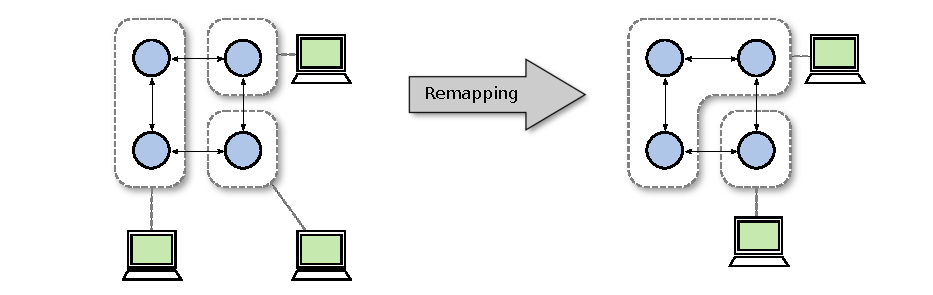
\includegraphics[width=\textwidth]{graphics/30_gvon_remapping}
  \caption{Redistribution of vertices to peers. The number of host of
    the graph is reduced from three hosts to two hosts.}
  \label{fig:gvon_remapping}
\end{figure}

Load balancing can be an issue when the communication topology is
changing during simulation execution. For example could the GoL
simulation add a new rule, which leads to a changed communication
topology for that in turn exists a better vertex mapping.  Even if the
performance of a network link drops, so that some hosts are not able
to reach accetable latency and bandwidth among each other, a
remapping can solve this problem at run-time.

A traditional field of application for remapping would be unbalanced
workload in the simulation application. Such an unbalanced state can
be recognized by monitoring and eliminated by remapping the workload
in a fair way.

Another issue is the failure of single cluster nodes and therefore
also a failure of hosts located on this nodes. Assuming, that the data
of hosts where check pointed, the hosted vertices of the failed host
can be adopted by another host, also at run-time.

The process of remapping is very similar to the mapping process of
Section~\ref{sec:mapping}.  It is also divided in two phases:
distribution and announcment. It has to be distinguished between
global and local remapping. A global remapping is a repetition of the
mapping process of Section~\ref{sec:mapping}.  Since, local remapping
situation is slightly different, because the hosts already own a set
of hosted vertices, it does not require a redistribution of all
vertices.  The distribution is more a swap or occupation of vertices.

\todo{Design summary}

\cleardoublepage

%%% Local Variables:
%%% TeX-master: "diplom"
%%% End:
